\chapter{Lecture 5: Input/Output in C++ and Strings}
\begin{center}
\textit{January 18, 2018}
\end{center}

\section{Hello World Revisited}
\begin{lstlisting}[style=cpp]
#include <iostream>
using namespace std;

int main() {
    cout << "Hello World!" << endl;
    return 0;
}
\end{lstlisting}
\begin{lstlisting}[style=bash]
g++ -std=c++14 hello.cc              # compiles to a.out
./a.out
g++ -std=c++14 hello.cc -o myprog    # compiles to myprog
\end{lstlisting}

\section{The Three Standard Streams}
Including \code{<iostream>} gives us three global variables:
\begin{center}
\begin{tabular}{@{}llp{0.5\textwidth}@{}}
\toprule
Variable & Type & Use \\
\midrule
\code{std::cout} & \code{ostream} & write to stdout with the \emph{output operator}
                                    \code{<<}: \code{cout << "Bla";} \\
\code{std::cin} & \code{istream} & read from stdin with the \emph{input operator}
                                  \code{>>}: \code{cin >> x;} \\
\code{std::cerr} & \code{ostream} & write to stderr: \code{cerr << "Error message";} \\
\bottomrule
\end{tabular}
\end{center}
As usual, \code{cout} is buffered and \code{cerr} is not.

\begin{example}
Add two numbers.
\begin{lstlisting}[style=cpp]
#include <iostream>
using namespace std;

int main() {
    int x, y;
    cin >> x >> y;
    cout << x + y << endl;
}
\end{lstlisting}
\end{example}

\section{Reading Input and Failure}
\code{cin >> x >> y} waits to read two \code{int}s, \emph{skipping whitespace}
(spaces, tabs, newlines). Reading an \code{int} stops at the first character that
cannot be part of an \code{int}.

\begin{itemize}
  \item If a read fails (bad input or EOF), the program keeps going, but all
        subsequent reads automatically fail as well.
  \item So after a read we should check whether it succeeded: after a read,
        \code{cin.fail()} is true if the read failed.
  \item If the read failed because of EOF, then \code{cin.fail()} and
        \code{cin.eof()} are both true.
\end{itemize}
(Reminder: Ctrl+D sends EOF; Ctrl+C kills the process.)

\begin{example}
Read all \code{int}s from stdin and echo them to stdout, one per line. Stop when
a read fails.
\begin{lstlisting}[style=cpp]
#include <iostream>
using namespace std;

int main() {
    int i;
    while (true) {
        cin >> i;
        if (cin.fail()) break;
        cout << i << endl;
    }
}
\end{lstlisting}
\end{example}

\subsection{Shortening the Loop}
C++ defines an automatic conversion from \code{istream} (e.g.\ \code{cin}) to
\code{bool}: \code{cin} converts to \code{true} if the last read did
\emph{not} fail. So \code{if (cin.fail())} can be written \code{if (!cin)}.

Next, recall that in C, if \code{int a = 21;} then \code{a >> 3} is a
\emph{right bit shift}: shift the bits of \code{a} three places to the right
(giving 2); \code{<<} is the left bit shift. In C++, operators can have multiple
meanings depending on the types of their operands; this is called
\textbf{operator overloading}. When the left operand is an \code{istream},
\code{>>} means ``read''.

\begin{important}[Expressions produce values]
\code{cin >> i} is an expression. Its \emph{side effect} is reading into
\code{i}; its \emph{value} is \code{cin} itself. That is why reads can be
cascaded: \code{cin >> x >> y} is \code{(cin >> x) >> y}.
\end{important}
\begin{center}
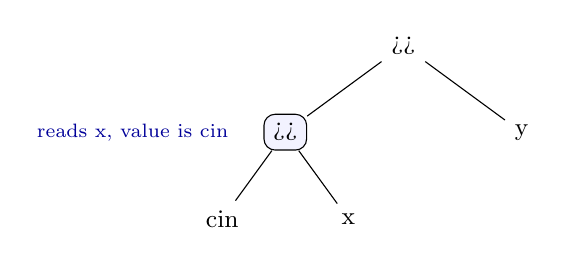
\begin{tikzpicture}[font=\small]
  \node (top) at (0,0) {\code{>{}>}};
  \node[draw,rounded corners,fill=blue!5] (in) at (-1.5,-1.1) {\code{>{}>}};
  \node (y) at (1.5,-1.1) {\code{y}};
  \node (cin) at (-2.3,-2.2) {\code{cin}};
  \node (x) at (-0.7,-2.2) {\code{x}};
  \draw (top) -- (in); \draw (top) -- (y); \draw (in) -- (cin); \draw (in) -- (x);
  \node[font=\scriptsize,blue!60!black,anchor=east] at (-2.1,-1.1) {reads \code{x}, value is \code{cin}};
\end{tikzpicture}
\end{center}

Putting it together, the loop shrinks step by step:
\begin{lstlisting}[style=cpp]
int main() {
    int i;
    while (true) {
        if (!(cin >> i)) break;   // read, then test the stream
        cout << i << endl;
    }
}

// ... and finally:
int main() {
    int i;
    while (cin >> i) {
        cout << i << endl;
    }
}
\end{lstlisting}

\begin{example}
Read all \code{int}s and echo them to stdout until EOF. Skip over non-integer
input.
\begin{lstlisting}[style=cpp]
#include <iostream>
using namespace std;

int main() {
    int i;
    while (true) {
        if (cin >> i) {
            cout << i << endl;
        } else {                  // read failed
            if (cin.eof()) break; // ... because of EOF: done
            cin.clear();          // acknowledge the failure (lower the fail flag)
            cin.ignore();         // skip the offending character
        }
    }
}
\end{lstlisting}
\code{cin.clear()} must come before \code{cin.ignore()}, because a stream in the
failed state ignores all operations.
\end{example}

The control flow of that loop:
\begin{center}
\begin{tikzpicture}[>=Stealth,font=\small,node distance=0.5cm and 1.2cm,
  act/.style={draw,rounded corners,fill=blue!5,minimum height=0.65cm},
  test/.style={draw,diamond,aspect=2.2,inner sep=1pt,fill=gray!8}]
  \node[act] (r) {\code{cin >{}> i}};
  \node[test,below=of r] (ok) {succeeded?};
  \node[act,right=of ok] (pr) {print \code{i}};
  \node[test,below=of ok] (eof) {\code{cin.eof()}?};
  \node[act,right=of eof] (stop) {\code{break}};
  \node[act,below=of eof] (cl) {\code{cin.clear(); cin.ignore();}};
  \draw[->] (r) -- (ok);
  \draw[->] (ok) -- node[above,font=\scriptsize]{yes} (pr);
  \draw[->] (ok) -- node[left,font=\scriptsize]{no} (eof);
  \draw[->] (eof) -- node[above,font=\scriptsize]{yes} (stop);
  \draw[->] (eof) -- node[left,font=\scriptsize]{no} (cl);
  \draw[->] (pr.north) |- (r.east);
  \draw[->] (cl.west) -- ++(-1.4,0) |- (r.west);
\end{tikzpicture}
\end{center}

\begin{aside}
\textbf{Look-up exercise: ignoring all of ``hello'' in one go.} \code{cin.ignore()}
skips one character, so the input \code{hello} costs five trips around the loop.
To skip the rest of the line:
\begin{lstlisting}[style=cpp]
#include <limits>
cin.ignore(numeric_limits<streamsize>::max(), '\n');
\end{lstlisting}
To skip just one whitespace-delimited word, read it into a \code{string} and
throw it away.
\end{aside}

\section{C++ Strings}
We have a \code{string} type in C++.

\begin{quote}
\textit{``What, no clapping? You do not feel the power of the string type.''}
--- Nomair Naeem
\end{quote}

In C, strings were simulated by null-terminated character arrays, which are
\begin{itemize}
  \item error prone (forget the \code{\textbackslash0}, overrun the array), and
  \item a memory-management burden (you must allocate enough space).
\end{itemize}
C++ has a \code{string} type. It is not built in; it comes from
\code{\#include <string>}. A C++ string grows as needed and manages its own
memory.

\begin{center}
\begin{tikzpicture}[>=Stealth,font=\small,x=0.6cm,
  ch/.style={draw,minimum width=0.6cm,minimum height=0.6cm,font=\ttfamily\small}]
  \node[anchor=east] at (-0.6,0) {C: \code{char s[6]}};
  \foreach \c [count=\k from 0] in {h,e,l,l,o} \node[ch] at (\k,0) {\c};
  \node[ch,fill=red!10] at (5,0) {\textbackslash0};
  \node[anchor=east] at (-0.6,-1.6) {C++: \code{string s}};
  \node[draw,fill=blue!5,minimum width=2.4cm,minimum height=0.8cm,align=center,font=\scriptsize] (obj) at (1.4,-1.6) {pointer, size 5,\\ capacity};
  \foreach \c [count=\k from 0] in {h,e,l,l,o} \node[ch] (h\k) at (\k+6,-1.6) {\c};
  \node[ch,draw=gray,text=gray] at (11,-1.6) {};
  \node[ch,draw=gray,text=gray] at (12,-1.6) {};
  \draw[->] (obj.east) -- (h0.west);
  \node[font=\scriptsize] at (9,-2.3) {heap buffer, grown and freed by \code{string}};
\end{tikzpicture}
\end{center}

\begin{lstlisting}[style=cpp]
string s = "hello";   // s is a C++ string; "hello" is a C string (const char*)
\end{lstlisting}
C strings are automatically converted to C++ strings, but not the other way
around (use \code{s.c\_str()} if you need a \code{const char*}).

\begin{center}
\begin{tabular}{@{}lll@{}}
\toprule
Operation & C & C++ \\
\midrule
equality & \code{strcmp(s1, s2) == 0} & \code{s1 == s2} \\
comparison & \code{strcmp} & \code{!=}, \code{<}, \code{<=}, \code{>}, \code{>=} \\
length & \code{strlen(s)} & \code{s.length()} \\
concatenation & \code{strcat(s1, s2)} & \code{s1 + s2}, \code{s1 += s2} \\
individual characters & \code{s[0]}, \dots & \code{s[0]}, \dots \\
\bottomrule
\end{tabular}
\end{center}

\begin{lstlisting}[style=cpp]
#include <iostream>
#include <string>
using namespace std;

int main() {
    string s;
    cin >> s;       // reads one whitespace-delimited word
    cout << s << endl;
}
\end{lstlisting}

To read a whole line (including spaces), use \code{getline(cin, s)}: it reads
into \code{s} everything up to (and discarding) the next newline.

Look up \code{std::string} (e.g.\ on cppreference) for more operations:
\code{substr}, \code{find}, \code{push\_back}, \code{insert}, \dots

\section{I/O Manipulators}
In C, \code{printf} uses format specifiers: \code{\%d} (int), \code{\%s}
(\code{char*}), \code{\%x} (int in hexadecimal). In C++ we use
\textbf{I/O manipulators} instead:
\begin{lstlisting}[style=cpp]
int i = 95;
cout << i;          // prints 95 in decimal
cout << hex << i;   // prints 5f (95 in hex)
cout << dec << i;   // back to decimal: 95
\end{lstlisting}
\code{hex} doesn't print anything; its side effect is to change the internal
state of the stream so that all subsequent integers print in hex. Manipulators
like \code{hex} and \code{dec} are therefore called \textbf{sticky}.

Other useful manipulators (many need \code{\#include <iomanip>}):
\begin{itemize}
  \item \code{boolalpha} / \code{noboolalpha}: print \code{bool}s as
        \code{true}/\code{false} rather than \code{1}/\code{0};
  \item \code{showpoint}, \code{setprecision(3)}, \code{fixed}: floating-point
        formatting;
  \item \code{setw(n)}, \code{setfill(c)}: field width and padding (\code{setw}
        is \emph{not} sticky --- it applies to the next item only);
  \item \code{skipws} / \code{noskipws}: whether \code{>>} skips whitespace.
\end{itemize}

\section{Other Sources of Data}
The stream abstraction can be used to read and write other sources of data. With
\code{\#include <fstream>} we get \code{ifstream} (input file stream) and
\code{ofstream} (output file stream). Using them is absolutely no different from
using \code{cin} and \code{cout} --- details next lecture.

\section*{Summary}
\begin{itemize}
  \item \code{cin >> x} reads (skipping whitespace), \code{cout << x} and
        \code{cerr << x} write.
  \item A failed read sets the fail bit; check with \code{cin.fail()},
        \code{cin.eof()} or just \code{if (cin >> x)}. Recover with
        \code{cin.clear()} then \code{cin.ignore()}.
  \item \code{cin >> x} evaluates to \code{cin}: this enables cascading and the
        idiom \code{while (cin >> i)}.
  \item Use \code{std::string}, not \code{char*}; \code{getline} reads lines.
  \item Manipulators (\code{hex}, \code{dec}, \code{boolalpha},
        \code{setprecision}, \dots) change stream state and are mostly sticky.
\end{itemize}
